\section{Results}\label{sec:results}

We evaluate whether learning the adjacency from traffic data improves
forecasting relative to a physical road-network graph, and under what
conditions. Unless noted otherwise, each value is the mean test RMSE over
five training seeds with the sample standard deviation in parentheses;
learned graphs are fitted once and shared across seeds. Improvements are
relative RMSE reductions with respect to the named reference. Statistical
qualifications follow Section~\ref{sec:stats}.

\subsection{Baselines: Physical Graph versus Graph-Free Control}\label{sec:res-physical}

\begin{table}[t]
\centering
\caption{T-GCN family: test RMSE (mean, sample standard deviation in
parentheses) over five seeds. PH1--PH4 correspond to $5$--$20$\,min
(Los-loop) and $15$--$60$\,min (SZ-Taxi). Bold: lowest mean in each dataset
block (not a significance claim).}
\label{tab:tgcn-main}
\small
\begin{tabular}{lcccc}
\toprule
Method & PH1 & PH2 & PH3 & PH4 \\
\midrule
\multicolumn{5}{l}{\textit{Los-loop (5\,min)}} \\
T-GCN (Physical) & 7.88 (0.28) & 8.13 (0.09) & 8.37 (0.17) & 8.66 (0.16) \\
T-GCN-NoSpatial & 5.25 (0.19) & 5.76 (0.08) & 6.11 (0.07) & 6.58 (0.12) \\
T-GCN-GSL & 5.86 (0.21) & 6.30 (0.06) & 6.66 (0.12) & 7.04 (0.09) \\
T-GCN-cGSL & 5.82 (0.23) & 6.35 (0.12) & 6.67 (0.11) & 7.09 (0.12) \\
T-GCN-MultiGSL & 4.84 (0.11) & 5.45 (0.14) & 5.94 (0.03) & 6.26 (0.03) \\
T-GCN-MultiGSL-Weighted & 4.83 (0.11) & 5.44 (0.13) & 5.93 (0.03) & 6.25 (0.03) \\
T-GCN-MultiGSL-Mix & \textbf{4.49 (0.14)} & \textbf{5.08 (0.15)} & \textbf{5.55 (0.16)} & \textbf{5.86 (0.07)} \\
\midrule
\multicolumn{5}{l}{\textit{SZ-Taxi (15\,min)}} \\
T-GCN (Physical) & 5.45 (0.11) & 5.55 (0.08) & 5.60 (0.05) & 5.63 (0.06) \\
T-GCN-NoSpatial & 4.12 (0.00) & 4.16 (0.01) & 4.19 (0.01) & 4.23 (0.01) \\
T-GCN-GSL & 4.28 (0.05) & 4.31 (0.03) & 4.33 (0.01) & 4.37 (0.02) \\
T-GCN-cGSL & 4.30 (0.03) & 4.34 (0.02) & 4.38 (0.03) & 4.41 (0.01) \\
T-GCN-MultiGSL & 4.13 (0.02) & 4.16 (0.00) & 4.20 (0.01) & 4.22 (0.00) \\
T-GCN-MultiGSL-Weighted & 4.13 (0.02) & 4.16 (0.00) & 4.20 (0.01) & 4.22 (0.00) \\
T-GCN-MultiGSL-Mix & \textbf{4.12 (0.02)} & \textbf{4.15 (0.01)} & \textbf{4.18 (0.00)} & \textbf{4.22 (0.01)} \\
\bottomrule
\end{tabular}
\end{table}

Table~\ref{tab:tgcn-main} reports the T-GCN family. The physical
road-network adjacency is the weakest configuration in its family in every
dataset--horizon cell. On Los-loop at PH1, T-GCN obtains $7.88\pm 0.28$
RMSE, while T-GCN-NoSpatial obtains $5.25\pm 0.19$ --- a $33.3\%$ relative
reduction when the physical graph is removed. NoSpatial beats Physical in
$5/5$ seeds in all eight cells.

\begin{table}[t]
\centering
\caption{GCN family: test RMSE (mean, sample standard deviation) over five
seeds. GCN-MultiGSL consumes the union of the three multi-lag graphs as one
static adjacency.}
\label{tab:gcn-main}
\small
\begin{tabular}{lcccc}
\toprule
Method & PH1 & PH2 & PH3 & PH4 \\
\midrule
\multicolumn{5}{l}{\textit{Los-loop (5\,min)}} \\
GCN (Physical) & 8.14 (0.11) & 8.54 (0.28) & 8.76 (0.26) & 8.76 (0.29) \\
GCN-NoSpatial & \textbf{4.88 (0.31)} & \textbf{5.60 (0.39)} & \textbf{6.02 (0.28)} & \textbf{6.26 (0.26)} \\
GCN-GSL & 7.83 (0.11) & 8.48 (0.21) & 8.45 (0.19) & 8.93 (0.12) \\
GCN-cGSL & 5.76 (0.20) & 6.33 (0.32) & 6.68 (0.25) & 6.88 (0.21) \\
GCN-MultiGSL & 9.78 (0.14) & 10.05 (0.16) & 10.24 (0.13) & 10.27 (0.11) \\
\midrule
\multicolumn{5}{l}{\textit{SZ-Taxi (15\,min)}} \\
GCN (Physical) & 5.96 (0.01) & 5.98 (0.00) & 5.99 (0.00) & 6.00 (0.00) \\
GCN-NoSpatial & \textbf{4.11 (0.00)} & \textbf{4.15 (0.00)} & \textbf{4.19 (0.00)} & \textbf{4.22 (0.00)} \\
GCN-GSL & 4.88 (0.01) & 4.91 (0.00) & 4.93 (0.01) & 4.96 (0.00) \\
GCN-cGSL & 4.64 (0.00) & 4.67 (0.00) & 4.70 (0.00) & 4.73 (0.00) \\
GCN-MultiGSL & 4.82 (0.01) & 4.85 (0.00) & 4.88 (0.01) & 4.90 (0.00) \\
\bottomrule
\end{tabular}
\end{table}

The GCN family (Table~\ref{tab:gcn-main}) shows the same pattern
(Los-loop PH1: GCN $8.14\pm 0.11$ vs.\ GCN-NoSpatial $4.88\pm 0.31$).
Figures~\ref{fig:rmsebars-tgcn} and~\ref{fig:rmsebars-gcn} summarize
five-seed mean RMSE for the T-GCN and GCN families separately.
Figure~\ref{fig:graphstruct} contrasts the dense physical adjacency with
the much sparser multi-lag union.

\begin{figure}[t]
\centering
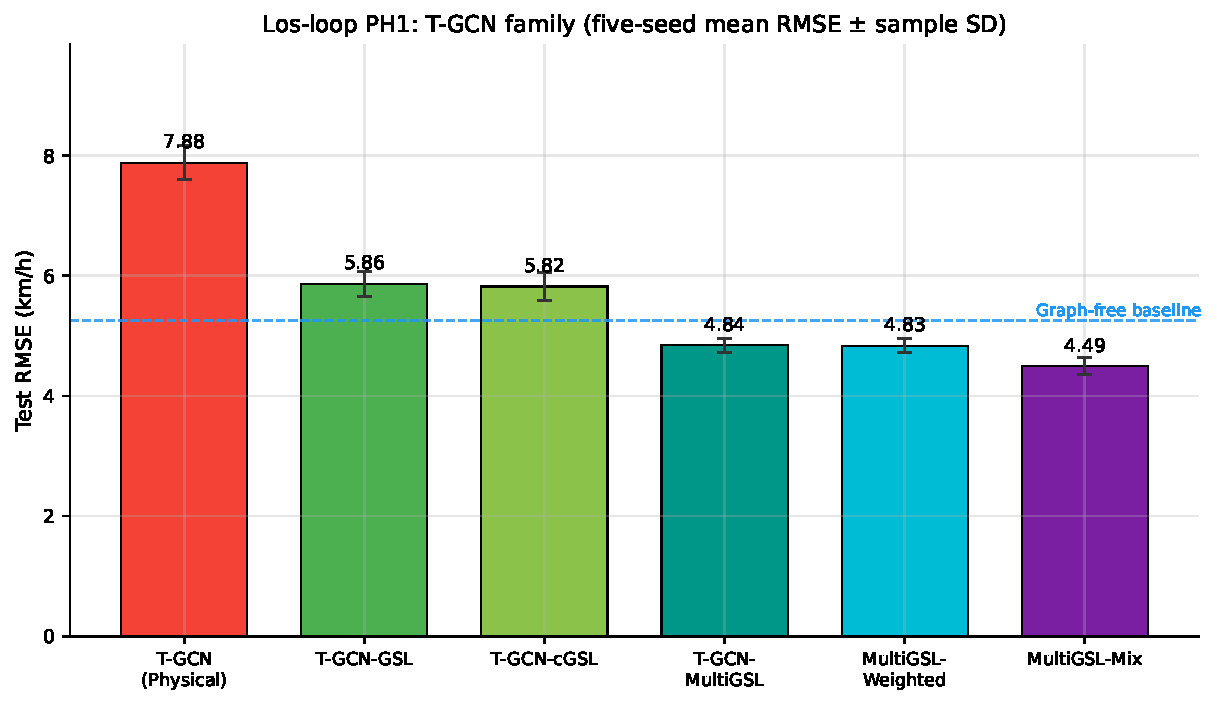
\includegraphics[width=0.95\linewidth]{figures/rmse_comparison_tgcn_los_ph1.pdf}
\caption{Los-loop PH1: T-GCN family, five-seed mean RMSE (whiskers: sample
SD). Dashed line: T-GCN-NoSpatial.}
\label{fig:rmsebars-tgcn}
\end{figure}

\begin{figure}[t]
\centering
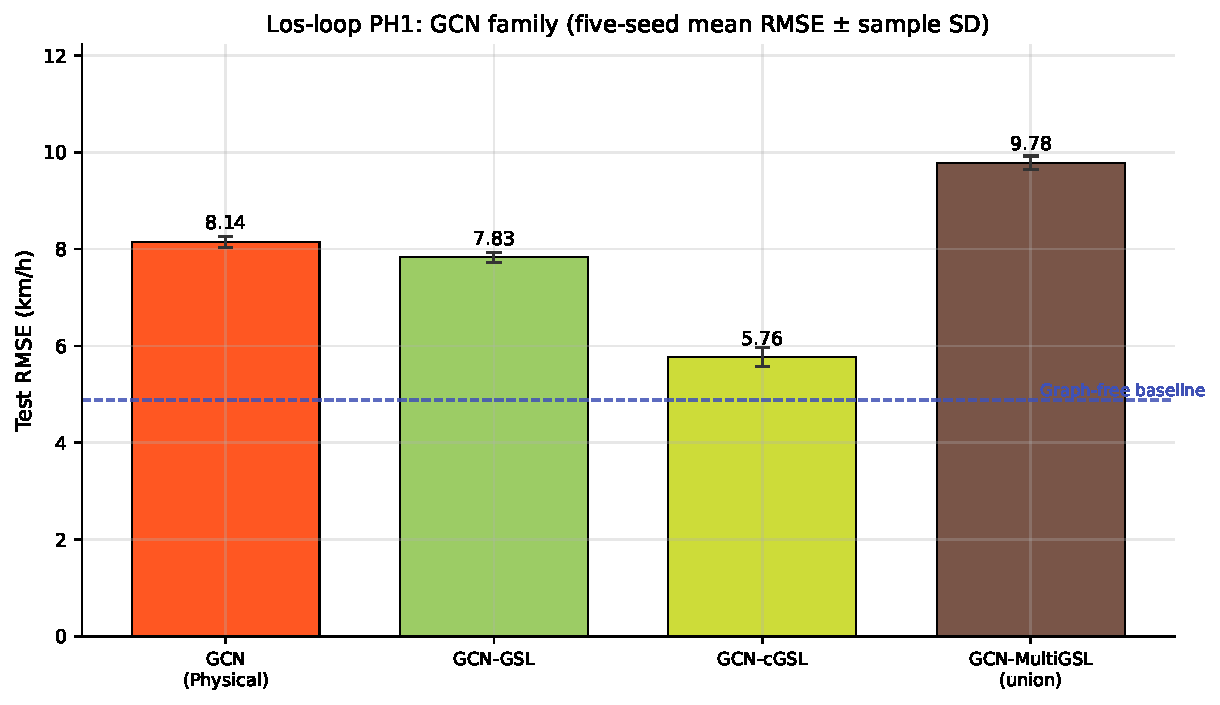
\includegraphics[width=0.95\linewidth]{figures/rmse_comparison_gcn_los_ph1.pdf}
\caption{Los-loop PH1: GCN family, five-seed mean RMSE (whiskers: sample
SD). Dashed line: GCN-NoSpatial.}
\label{fig:rmsebars-gcn}
\end{figure}

\begin{figure}[t]
\centering
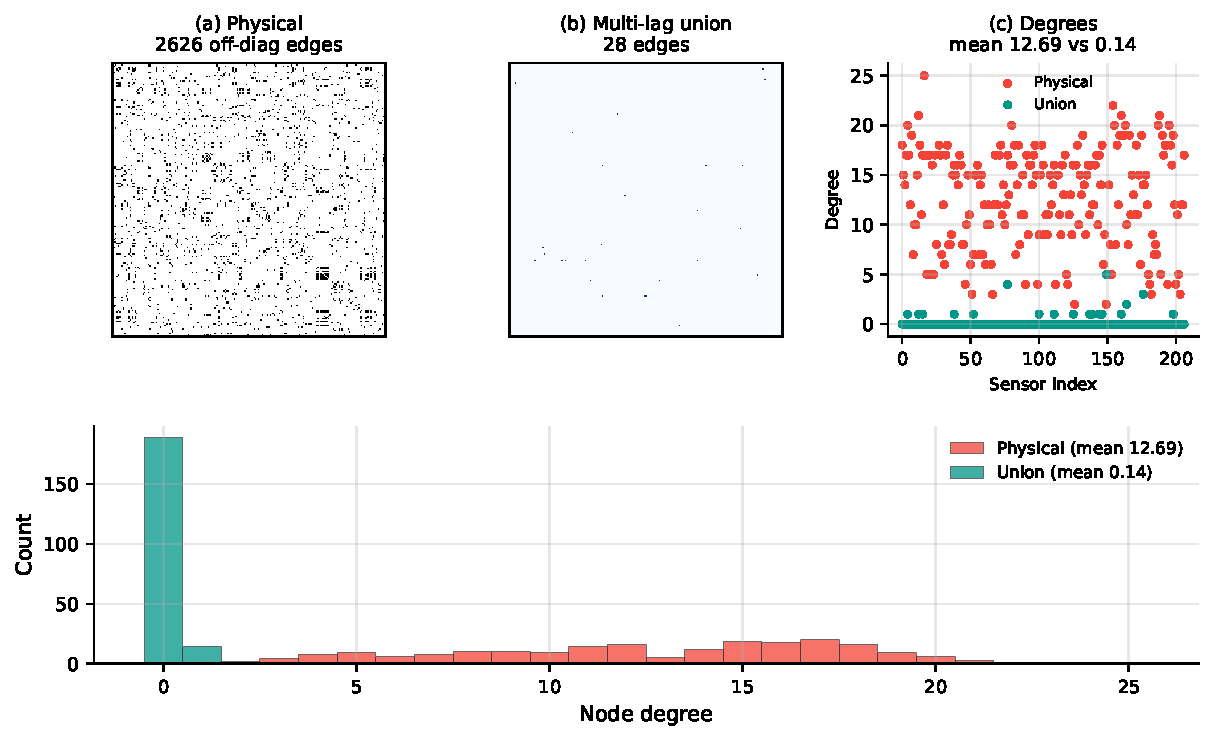
\includegraphics[width=0.98\linewidth]{figures/graph_structure_los.pdf}
\caption{Los-loop graph structure: (a) physical adjacency ($2626$
off-diagonal edges; mean degree $12.69$); (b) multi-lag union after
consumer thresholding ($28$ edges; mean degree $0.14$); (c) node degrees.
Learned graphs are statistical dependency estimates, not causal maps.}
\label{fig:graphstruct}
\end{figure}

\subsection{Contemporaneous Learned Graphs (GSL and cGSL)}\label{sec:res-single}

Replacing the physical adjacency with a single contemporaneous DAGMA graph
improves on Physical in most T-GCN cells but does not surpass the
graph-free control. On Los-loop PH1, T-GCN-GSL and T-GCN-cGSL obtain
$5.86\pm 0.21$ and $5.82\pm 0.23$, about $26\%$ better than Physical yet
about $11\%$ worse than NoSpatial. Neither contemporaneous graph beats
NoSpatial in any dataset$\times$horizon cell. For GCN, cGSL is better than
directed GSL on Los-loop ($5.76$ vs.\ $7.83$) but still worse than
GCN-NoSpatial; for T-GCN, GSL and cGSL are nearly indistinguishable.

\subsection{Is the Gain Only Sparsity?}\label{sec:res-controls}

The physical graph is dense (order $10^3$ off-diagonal edges on Los-loop),
while single contemporaneous GSL uses $28$ edges and the multi-lag
construction uses $30$ lag slots (union $28$). To test whether any gain
from a learned sparse graph is only an edge-count effect, we compare
graphs at a **matched $30$-edge budget** on Los-loop PH1
(Table~\ref{tab:controls}; Figure~\ref{fig:sparsity}).

\begin{table}[t]
\centering
\caption{Matched-sparsity and capacity controls on Los-loop at PH1 only.
Five seeds for graph rows; capacity rows are single-seed (seed 42).}
\label{tab:controls}
\small
\begin{tabular}{lccc}
\toprule
Configuration & RMSE & Budget / params & vs NoSpatial \\
\midrule
RandTop30 & 6.10 (0.12) & 30 random edges & $+16.1\%$ \\
CorrTop30 & 5.39 (0.10) & 30 top-$|$Pearson$|$ & $+2.6\%$ \\
T-GCN-NoSpatial & 5.25 (0.19) & identity & --- \\
T-GCN-MultiGSL & 4.84 (0.11) & 30 DAGMA lag slots & $-7.8\%$ \\
T-GCN-MultiGSL-Mix & 4.49 (0.14) & same graphs, gated & $-14.5\%$ \\
\midrule
NoSpatial $h{=}64$ (seed 42) & 5.14 & $12{,}672$ params & --- \\
NoSpatial $h{=}74$ (seed 42) & 5.14 & $16{,}872$ params & $\approx 0\%$ \\
Mix (seed 42) & 4.46 & $17{,}091$ params & $-13.3\%$ \\
\bottomrule
\end{tabular}
\end{table}

At this matched budget, a random $30$-edge graph is **worse** than using
no graph (RandTop30 $6.10\pm 0.12$ vs.\ NoSpatial $5.25\pm 0.19$), and a
top-correlation $30$-edge graph is only slightly better than random but
still **worse** than NoSpatial (CorrTop30 $5.39\pm 0.10$). The DAGMA
multi-lag graphs with the same $30$-edge budget, when used with
lag-aligned T-GCN (MultiGSL) or gating (Mix), **beat** NoSpatial. Sparsity
alone therefore does not explain the multi-lag result on this cell; the
placement of the learned edges (and how they are used) matters. A
capacity-matched graph-free model (hidden $74$; single seed) stays near
$5.14$ RMSE, so the gate's extra parameters do not explain Mix's gain.

\begin{figure}[t]
\centering
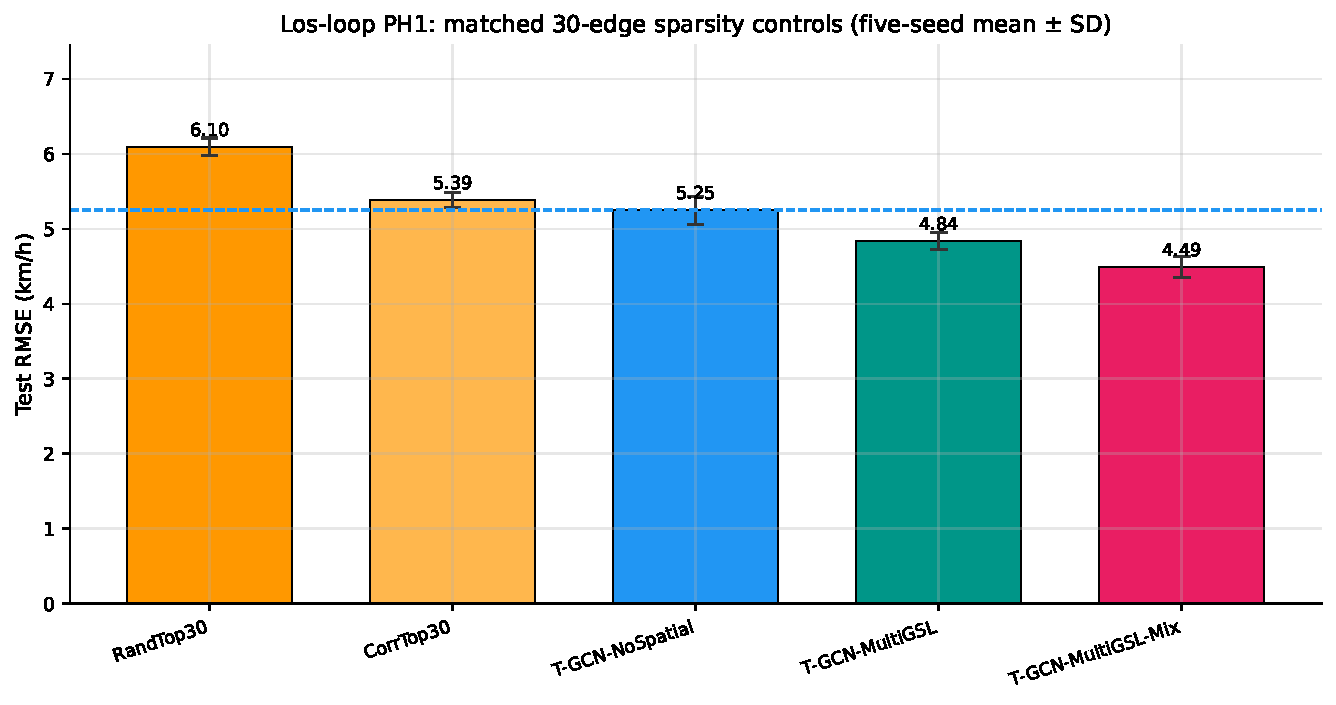
\includegraphics[width=0.95\linewidth]{figures/sparsity_controls_los_ph1.pdf}
\caption{Matched-sparsity controls on Los-loop at PH1 (five-seed mean $\pm$
sample SD). RandTop30 and CorrTop30 use a $30$-edge budget; MultiGSL and
Mix use the DAGMA multi-lag graphs. Dashed line: T-GCN-NoSpatial.}
\label{fig:sparsity}
\end{figure}

\subsection{Multi-Lag Learned Graphs}\label{sec:res-multilag}

On Los-loop the multi-lag graphs are informative ($12$/$3$/$15$ edges by
lag; union $28$). T-GCN-MultiGSL yields $4.84\pm 0.11$ at PH1; Mix improves
to $4.49\pm 0.14$. Relative to NoSpatial, Mix reduces RMSE by $14.5\%$,
$11.9\%$, $9.2\%$, and $10.9\%$ at PH1--PH4 (Table~\ref{tab:tgcn-main};
$5/5$ paired seeds). Relative to Physical T-GCN: $43.0\%$, $37.6\%$,
$33.7\%$, $32.3\%$. Paired $t$-tests for Mix vs NoSpatial give
$p\approx 0.0015$, $0.0015$, $0.0008$, $<10^{-4}$ (reference only;
Section~\ref{sec:stats}).

\begin{figure}[t]
\centering
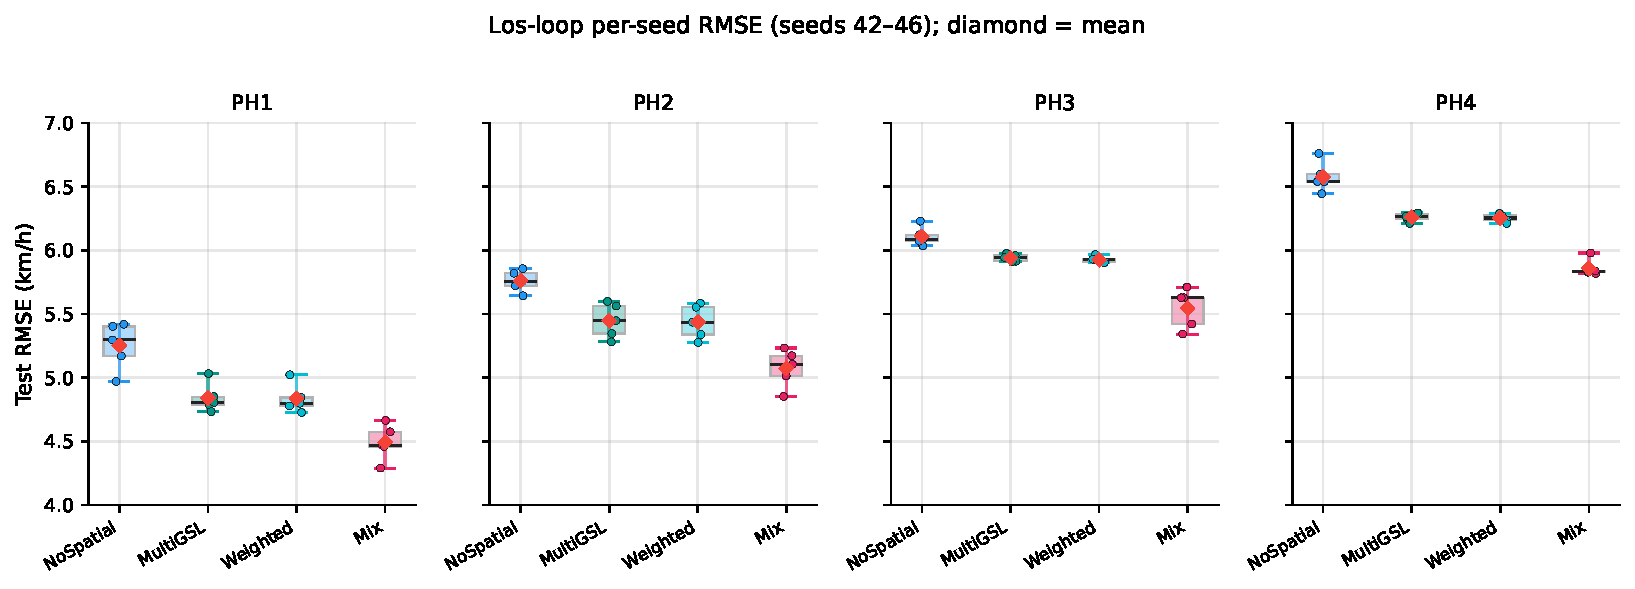
\includegraphics[width=0.98\linewidth]{figures/perseed_rmse_los.pdf}
\caption{Los-loop per-seed test RMSE for the multi-lag use ladder (seeds
42--46). Diamonds mark five-seed means matching Table~\ref{tab:tgcn-main}.}
\label{fig:perseed}
\end{figure}

Figure~\ref{fig:perseed} shows the per-seed distributions: Mix has the
lowest mean RMSE among the evaluated configurations on Los-loop at all four
horizons. Weighted is essentially tied with the fixed MultiGSL assignment
(differences $\le 0.01$ RMSE).

\begin{figure}[t]
\centering
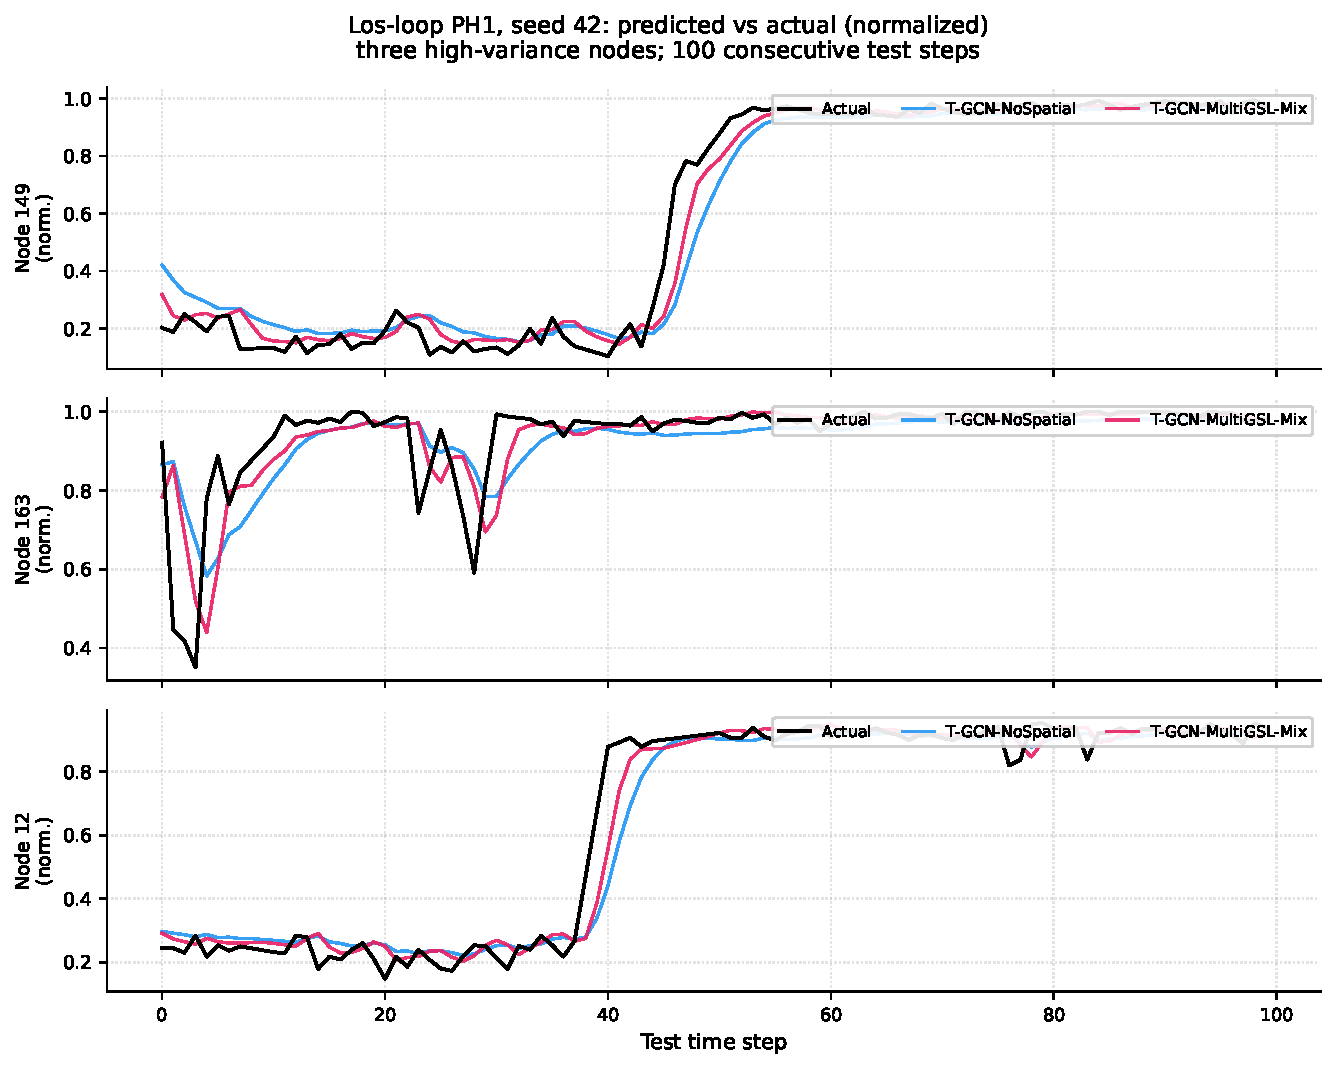
\includegraphics[width=0.98\linewidth]{figures/pred_vs_actual_los_ph1.pdf}
\caption{Predicted versus actual speed on Los-loop (PH1, seed $42$) for
three high-variance nodes (100 test steps). Each row overlays ground truth
with T-GCN-NoSpatial and T-GCN-MultiGSL-Mix (normalized scale).}
\label{fig:predvsact}
\end{figure}

When the same multi-lag artifacts are merged into one static union for
GCN-MultiGSL, error is $9.78\pm 0.14$ on Los-loop PH1 --- worse than the
physical GCN and more than twice T-GCN-MultiGSL on the same graphs
(Table~\ref{tab:gcn-main}). The union retains $28$ of $30$ lag slots; the
comparison does not isolate consumption from backbone differences, but
shows that multi-lag graphs are not automatically beneficial once estimated.

\subsection{Dataset Dependence and Temporal Resolution}\label{sec:res-boundaries}

On SZ-Taxi the multi-lag fit retains only two lagged edges. Mix vs
NoSpatial differs by at most $0.015$ RMSE ($\le 0.34\%$). The Los-loop
result does not transfer under this construction.

\paragraph{Los-loop at 15-minute sampling (resolution control).}
To test whether SZ-Taxi's weak separation could be an artifact of coarser
sampling, Los-loop was resampled to $15$-minute steps. PH1--4 then
correspond to $15$, $30$, $45$, and $60$ minutes ahead (wall-clock
equivalent to PH3/6/9/12 on the $5$-minute grid, but not the same as
direct PH3/6/9/12 evaluation on $5$-minute data). Mix vs NoSpatial:
$27.4\%$, $21.4\%$, $19.8\%$, $16.1\%$ relative reductions with $5/5$ seed
wins (Table~\ref{tab:los15}). Temporal resolution alone does not explain
SZ-Taxi; lag-structure recovery differs sharply ($30$ vs.\ $2$ slots).

\begin{table}[t]
\centering
\caption{Los-loop temporal-resolution variant at $15$-minute sampling.
PH $k$ denotes $15k$ minutes ahead; not comparable to PH $k$ of the
$5$-minute series. Five seeds; sample SD (ddof$=1$).}
\label{tab:los15}
\small
\begin{tabular}{lcccc}
\toprule
Method & PH1 (15\,min) & PH2 (30\,min) & PH3 (45\,min) & PH4 (60\,min) \\
\midrule
T-GCN-NoSpatial & 8.600 (0.279) & 9.311 (0.220) & 10.048 (0.083) & 10.460 (0.220) \\
T-GCN-MultiGSL & 7.246 (0.333) & 8.571 (0.365) & 9.112 (0.087) & 9.756 (0.234) \\
T-GCN-MultiGSL-Mix & \textbf{6.240 (0.209)} & \textbf{7.322 (0.378)} & \textbf{8.063 (0.227)} & \textbf{8.777 (0.364)} \\
\midrule
Mix vs NoSpatial & $-27.4\%$ & $-21.4\%$ & $-19.8\%$ & $-16.1\%$ \\
Mix wins (of 5) & 5 & 5 & 5 & 5 \\
\bottomrule
\end{tabular}
\end{table}

\subsection{Summary of Findings}\label{sec:res-summary}

\begin{enumerate}
\item Learning $\mathbf{A}$ from data can improve on the physical graph,
but a graph-free control is necessary to judge the contribution of spatial
structure.
\item A single contemporaneous learned graph does not beat the graph-free
control on these benchmarks.
\item Multi-lag graphs help on Los-loop when used in a lag-aligned way in
T-GCN; Mix has the lowest mean RMSE among evaluated multi-lag variants.
Sparsity alone does not explain this gain on the matched-budget cell.
\item The benefit is dataset-dependent: SZ-Taxi shows little separation
from the graph-free baseline.
\end{enumerate}

